\begin{savequote}[75mm]
The feeling is less like an ending than just another starting point.
\qauthor{Chuck Palahniuk}
\end{savequote}

\chapter{Combined Run 1 $H\rightarrow WW^{*}\rightarrow \ell\nu\ell\nu$ results}

\section{Introduction}

In the final statistical analysis of \HWWfull, the dedicated gluon-gluon fusion and vector boson fusion sensitive signal regions are all combined into a single fit to determine the main parameters of interest, the Higgs signal strength $\mu$ and mass $m_H$. This chapter presents the combined interpretation of results in the \HWWfull analysis for gluon fusion and vector boson fusion Higgs production. First, the results of the dedicated gluon fusion search are presented. These results are an extension of the discovery analysis (presented in chapter 4) to the full Run 1 dataset. Next, a comparison of the individual production mode signal strengths ($\mu_{\ggF}$ and $\mu_{\VBF}$) and a measurement of the combined signal strength ($\mu$) are shown. Then, the measured values of the Higgs couplings to fermions and vector bosons are presented. Finally, the cross section measurement for ggF and VBF production are shown. 

\section{Results of dedication gluon fusion \HWWfull analysis}

The analysis of gluon fusion Higgs production which led to the discovery of the Higgs, as presented in chapter 4, was also extended to the full Run 1 dataset. This new result included many improvements, such as more robust $\MET$ definitions, a lower sub-leading lepton $\pT$ threshold ($10 \GeV$), and the inclusion of the same flavor final states~\cite{WW2015}. This section presents the results from the gluon fusion dedicated signal regions in the full Run 1 data. A special focus is placed on the results from the same flavor final state channels. 

\subsection{Results in same flavor ($ee/\mu\mu$) final states}

Final states of the \HWWfull channel where both leptons have the same flavor ($ee/\mu\mu$) were not included in the discovery result due to increased pileup conditions in the $\sqrt{s} = 8 \TeV$ data. Dedicated techniques for background reduction in the same flavor final states were developed, as described in section~\ref{sec:sameflavor}. The results shown in this section are the first published results using the same flavor channels in the $\HWW$ analysis. 

\begin{table}[h!]
\centering
\captionsetup{justification=centering}

%\begin{tabular*}{0.480\textwidth}{p{0.075\textwidth} p{0.180\textwidth} l}
\hspace{-10pt}
\begin{tabular}{|c|c|c|c|c|}
\hline
 & $N_{\rm obs}$ & $N_{\rm bkg}$ & $N_{\rm ggF}$ & $N_{\rm VBF}$ \\ \hline
$\Njet = 0$ & $1108$ & $1040 \pm 40$ & $77 \pm 15$ & $2.4 \pm 1.7$ \\ \hline
$\Njet = 1$ & $467$ & $427 \pm 21$ & $22 \pm 6$ & $3.6 \pm 1.8$ \\ \hline
\end{tabular}

\caption{
Summary of post-fit yields in ggF dedicated signal regions for the $ee/\mu\mu$ final states~\cite{WW2015}. 
}
\label{tab:ggF_sf}
\end{table}

Table~\ref{tab:ggF_sf} shows the background estimate, expected signal yield, and event count in data for the same flavor channels in the $\Njet \leq 1$ signal regions. The dedicated same flavor background reduction techniques allow this channel to preserve a signal to background ratio ($0.074$ for $\Njet = 0$) similar to that of the different flavor channels ($0.087$ for $\Njet = 0$). Table~\ref{tab:ggF_sf_bkg} shows the breakdown of the background composition in the same flavor channels. It can be seen there that after using background reduction requirements, the $\ZDY$ background only contributes approximately $5\%$ ($7\%$) of the total background in the $\Njet = 0\,(1)$ bin. 

\begin{table}[h!]
\centering
\captionsetup{justification=centering}

%\begin{tabular*}{0.480\textwidth}{p{0.075\textwidth} p{0.180\textwidth} l}
\hspace{-10pt}
\begin{tabular}{|c|c|c|}
\hline
Background & $\Njet = 0$ & $\Njet = 1$ \\ \hline
$\NWW$ & $740 \pm 40$ & $184 \pm 15$ \\ \hline
$\Nt$ & $39 \pm 3$ & $46 \pm 4$ \\ \hline
$\Nttbar$ & $65 \pm 5$ & $119 \pm 10$ \\ \hline
$\NWj$ & $82 \pm 16$ & $19 \pm 4$ \\ \hline
$\Njj$ & $2 \pm 0.5$ & $0.2 \pm 0.1$ \\ \hline
$\NVV$ & $64 \pm 7$ & $31 \pm 4$ \\ \hline
$\NDY$ & $50 \pm 21$ & $28 \pm 12$ \\ \hline
\end{tabular}

\caption{
Post-fit background composition in ggF dedicated signal regions for the $ee/\mu\mu$ final states~\cite{WW2015}. 
}
\label{tab:ggF_sf_bkg}
\end{table}

Figure~\ref{fig:ggF_mT_sf} shows the final $\mTH$ distribution in data for the $\Njet \leq 1$ same flavor channels. The data is very consistent with the Higgs hypothesis and it can be seen that the same flavor channels are indeed sensitive to gluon fusion production of the Higgs. 

\begin{figure}[h!]
  %\vspace{20pt}
  \centering
  \captionsetup{justification=centering}

  %\hspace*{-32pt}
  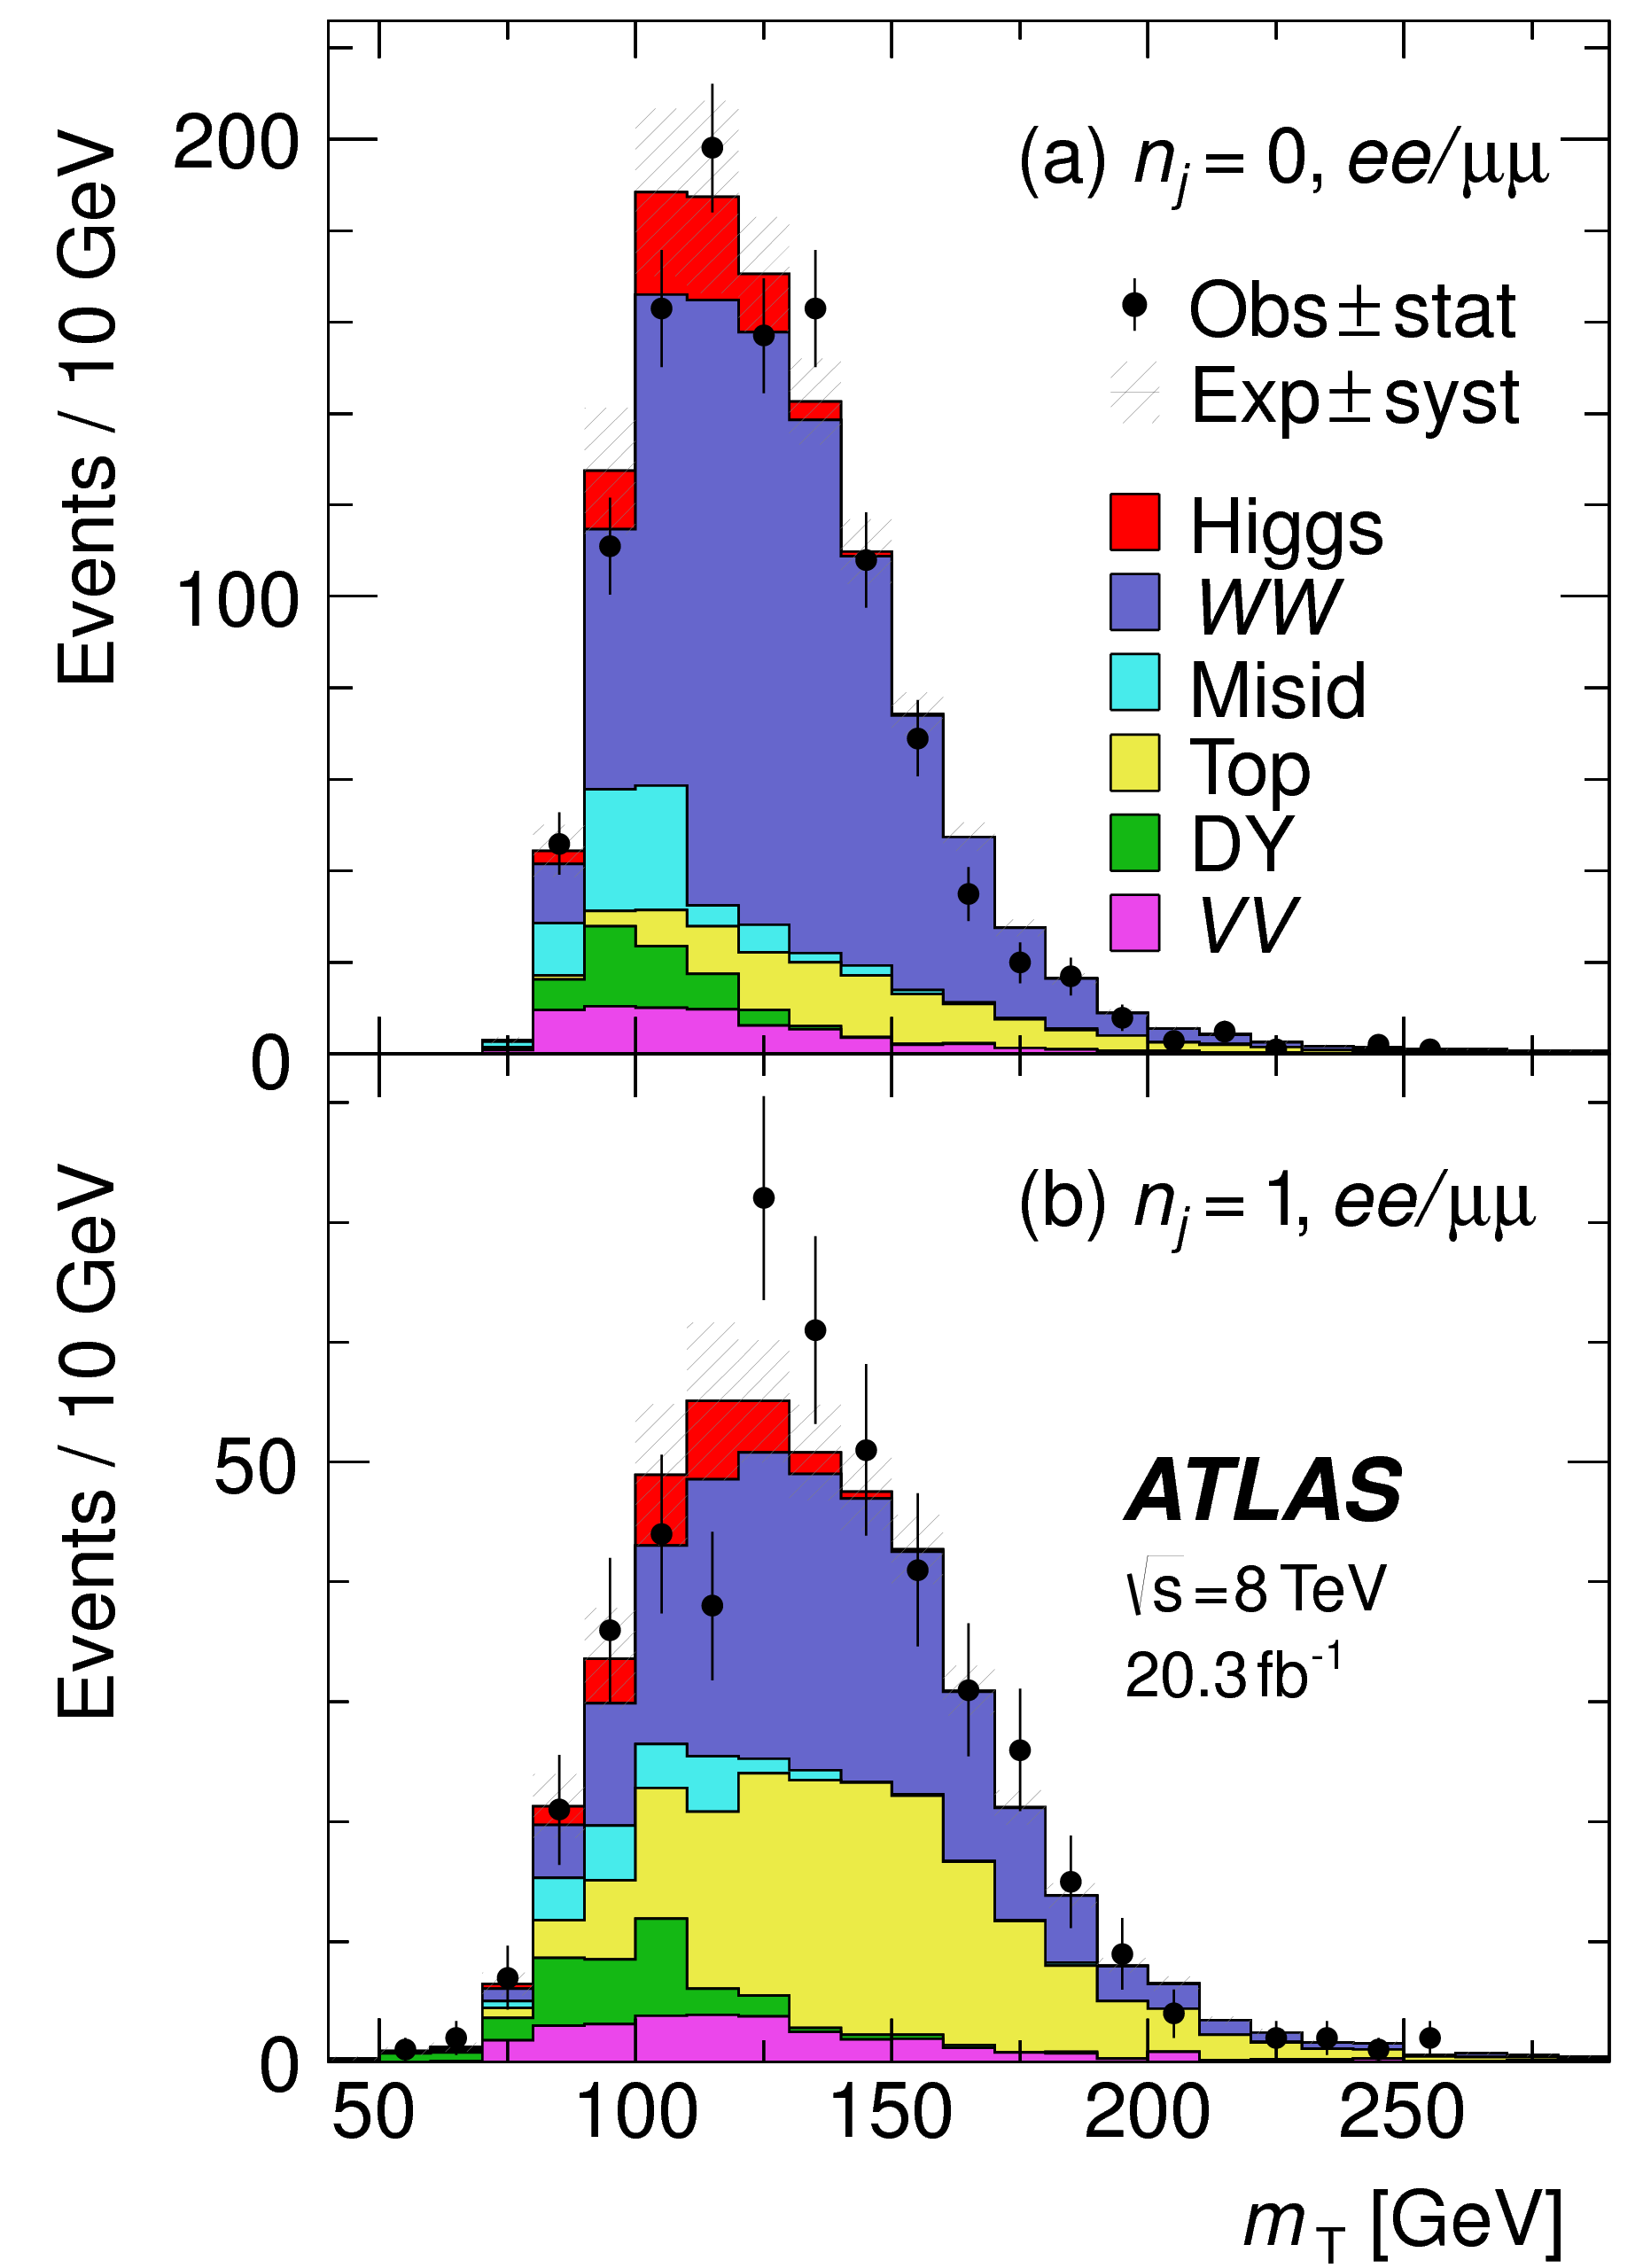
\includegraphics[width=0.6\textwidth]{figures/ggF_mT_sameflavor}
  \caption{Post-fit $\mTH$ distribution in the $\Njet \leq 1$ regions for the same flavor ($ee/\mu\mu$) final states~\cite{WW2015}.}
  \label{fig:ggF_mT_sf}
\end{figure}

\subsection{Combined gluon fusion results}

Table~\ref{tab:fitregions} shows the individual signal regions that were input into the final statistical fit. The ggF dedicated bins use $\mTH$ as their discriminating variable and are separated into bins of $\pT$ of the subleading lepton as well. 

%The VBF dedicated bin uses the $\bdt$ distribution as its final discriminant. 

\begin{table*}[tb!]
\centering%
\captionsetup{justification=centering}

%--------------------------------------------------------------------------------
\begin{tabular*}{\textwidth}{
  p{0.3\textwidth}
  l %p{0.100\textwidth}
  l %p{0.100\textwidth}
  l
  c
  c
}
\\
\dbline
\multicolumn{4}{c}{SR category $i$}
&
&\multicolumn{1}{l}{\multirow{2}{*}{Fit var.}}
\\
\clineskip%
\cline{1-4}%
\clineskip%
$\Njet$, flavor
&${\otimes\,}\mll$
&${\otimes\,}\pTsublead$
&${\otimes\,}\ell_2$
&
&
\\
\sgline
$\NjetEQzero$ \\
\quad $\DFchan$     &${\otimes\,}[10,30,55]$ &${\otimes\,}[10,15,20,\infty]$ &${\otimes\,}[e,\mu]$ &&$\mTH$ \\
\quad $\SFchan$     &${\otimes\,}[12,55]$    &${\otimes\,}[10,\infty]$       &                     &&$\mTH$ \\
\sgline
$\NjetEQone$ \\
\quad $\DFchan$     &${\otimes\,}[10,30,55]$ &${\otimes\,}[10,15,20,\infty]$ &${\otimes\,}[e,\mu]$ &&$\mTH$ \\
\quad $\SFchan$     &${\otimes\,}[12,55]$    &${\otimes\,}[10,\infty]$       &                     &&$\mTH$ \\
\sgline
$\NjetGEtwo$ ggF \\
\quad $\DFchan$     &${\otimes\,}[10,55]$    &${\otimes\,}[10,\infty]$       &                     &&$\mTH$ \\
\sgline
\multicolumn{2}{l}{$\NjetGEtwo$ VBF} \\
\quad $\DFchan$     &${\otimes\,}[10,50]$    &${\otimes\,}[10,\infty]$       &                     &&$\bdt$ \\
\quad $\SFchan$     &${\otimes\,}[12,50]$    &${\otimes\,}[10,\infty]$       &                     &&$\bdt$ \\
\end{tabular*}
\caption{
  All signal regions definitions input into final statistical fit~\cite{WW2015}.
}
\label{tab:fitregions}
\end{table*}
%eof

Table~\ref{tab:final-yields} shows the yields in the various signal regions in both data and expected signal and backgrounds. The yields for signal and background are all scaled according to the final normalizations calculated in the fit. 

\begin{table}[h!]
\centering
\captionsetup{justification=centering}

%\begin{tabular*}{0.480\textwidth}{p{0.075\textwidth} p{0.180\textwidth} l}
\hspace{-10pt}
\begin{tabular}{|c|c|c|c|c|}
\hline
 & $N_{\rm obs}$ & $N_{\rm bkg}$ & $N_{\rm ggF}$ & $N_{\rm VBF}$ \\ \hline
$\Njet = 0$ & $3750$ & $3430 \pm 90$ & $300 \pm 50$ & $8 \pm 4$ \\ \hline
$\Njet = 1$ & $1596$ & $1470 \pm 40$ & $102 \pm 26$ & $17 \pm 5$ \\ \hline
$\Njet \geq 2$, $\rm ggF$ $e\mu$ & $1017$ & $960 \pm 40$ & $37 \pm 11$ & $13 \pm 1.4$ \\ \hline
$\Njet \geq 2$, $\rm VBF$ & $130$ & $99 \pm 9$ & $7.7 \pm 2.6$ & $21 \pm 3$ \\ \hline
\end{tabular}

\caption{
Post-fit yields in the both ggF and VBF dedicated signal regions with all lepton flavor final states combined~\cite{WW2015}. 
}
\label{tab:final-yields}
\end{table}

Figure~\ref{fig:ggF-mT} shows the final post-fit $\mTH$ distribution in the $\Njet \leq 1$ regions. The data are very consistent with the hypothesis of ggF Higgs production. 
%
\begin{figure}[h!]
  %\vspace{20pt}
  \centering
  \captionsetup{justification=centering}

  %\hspace*{-32pt}
  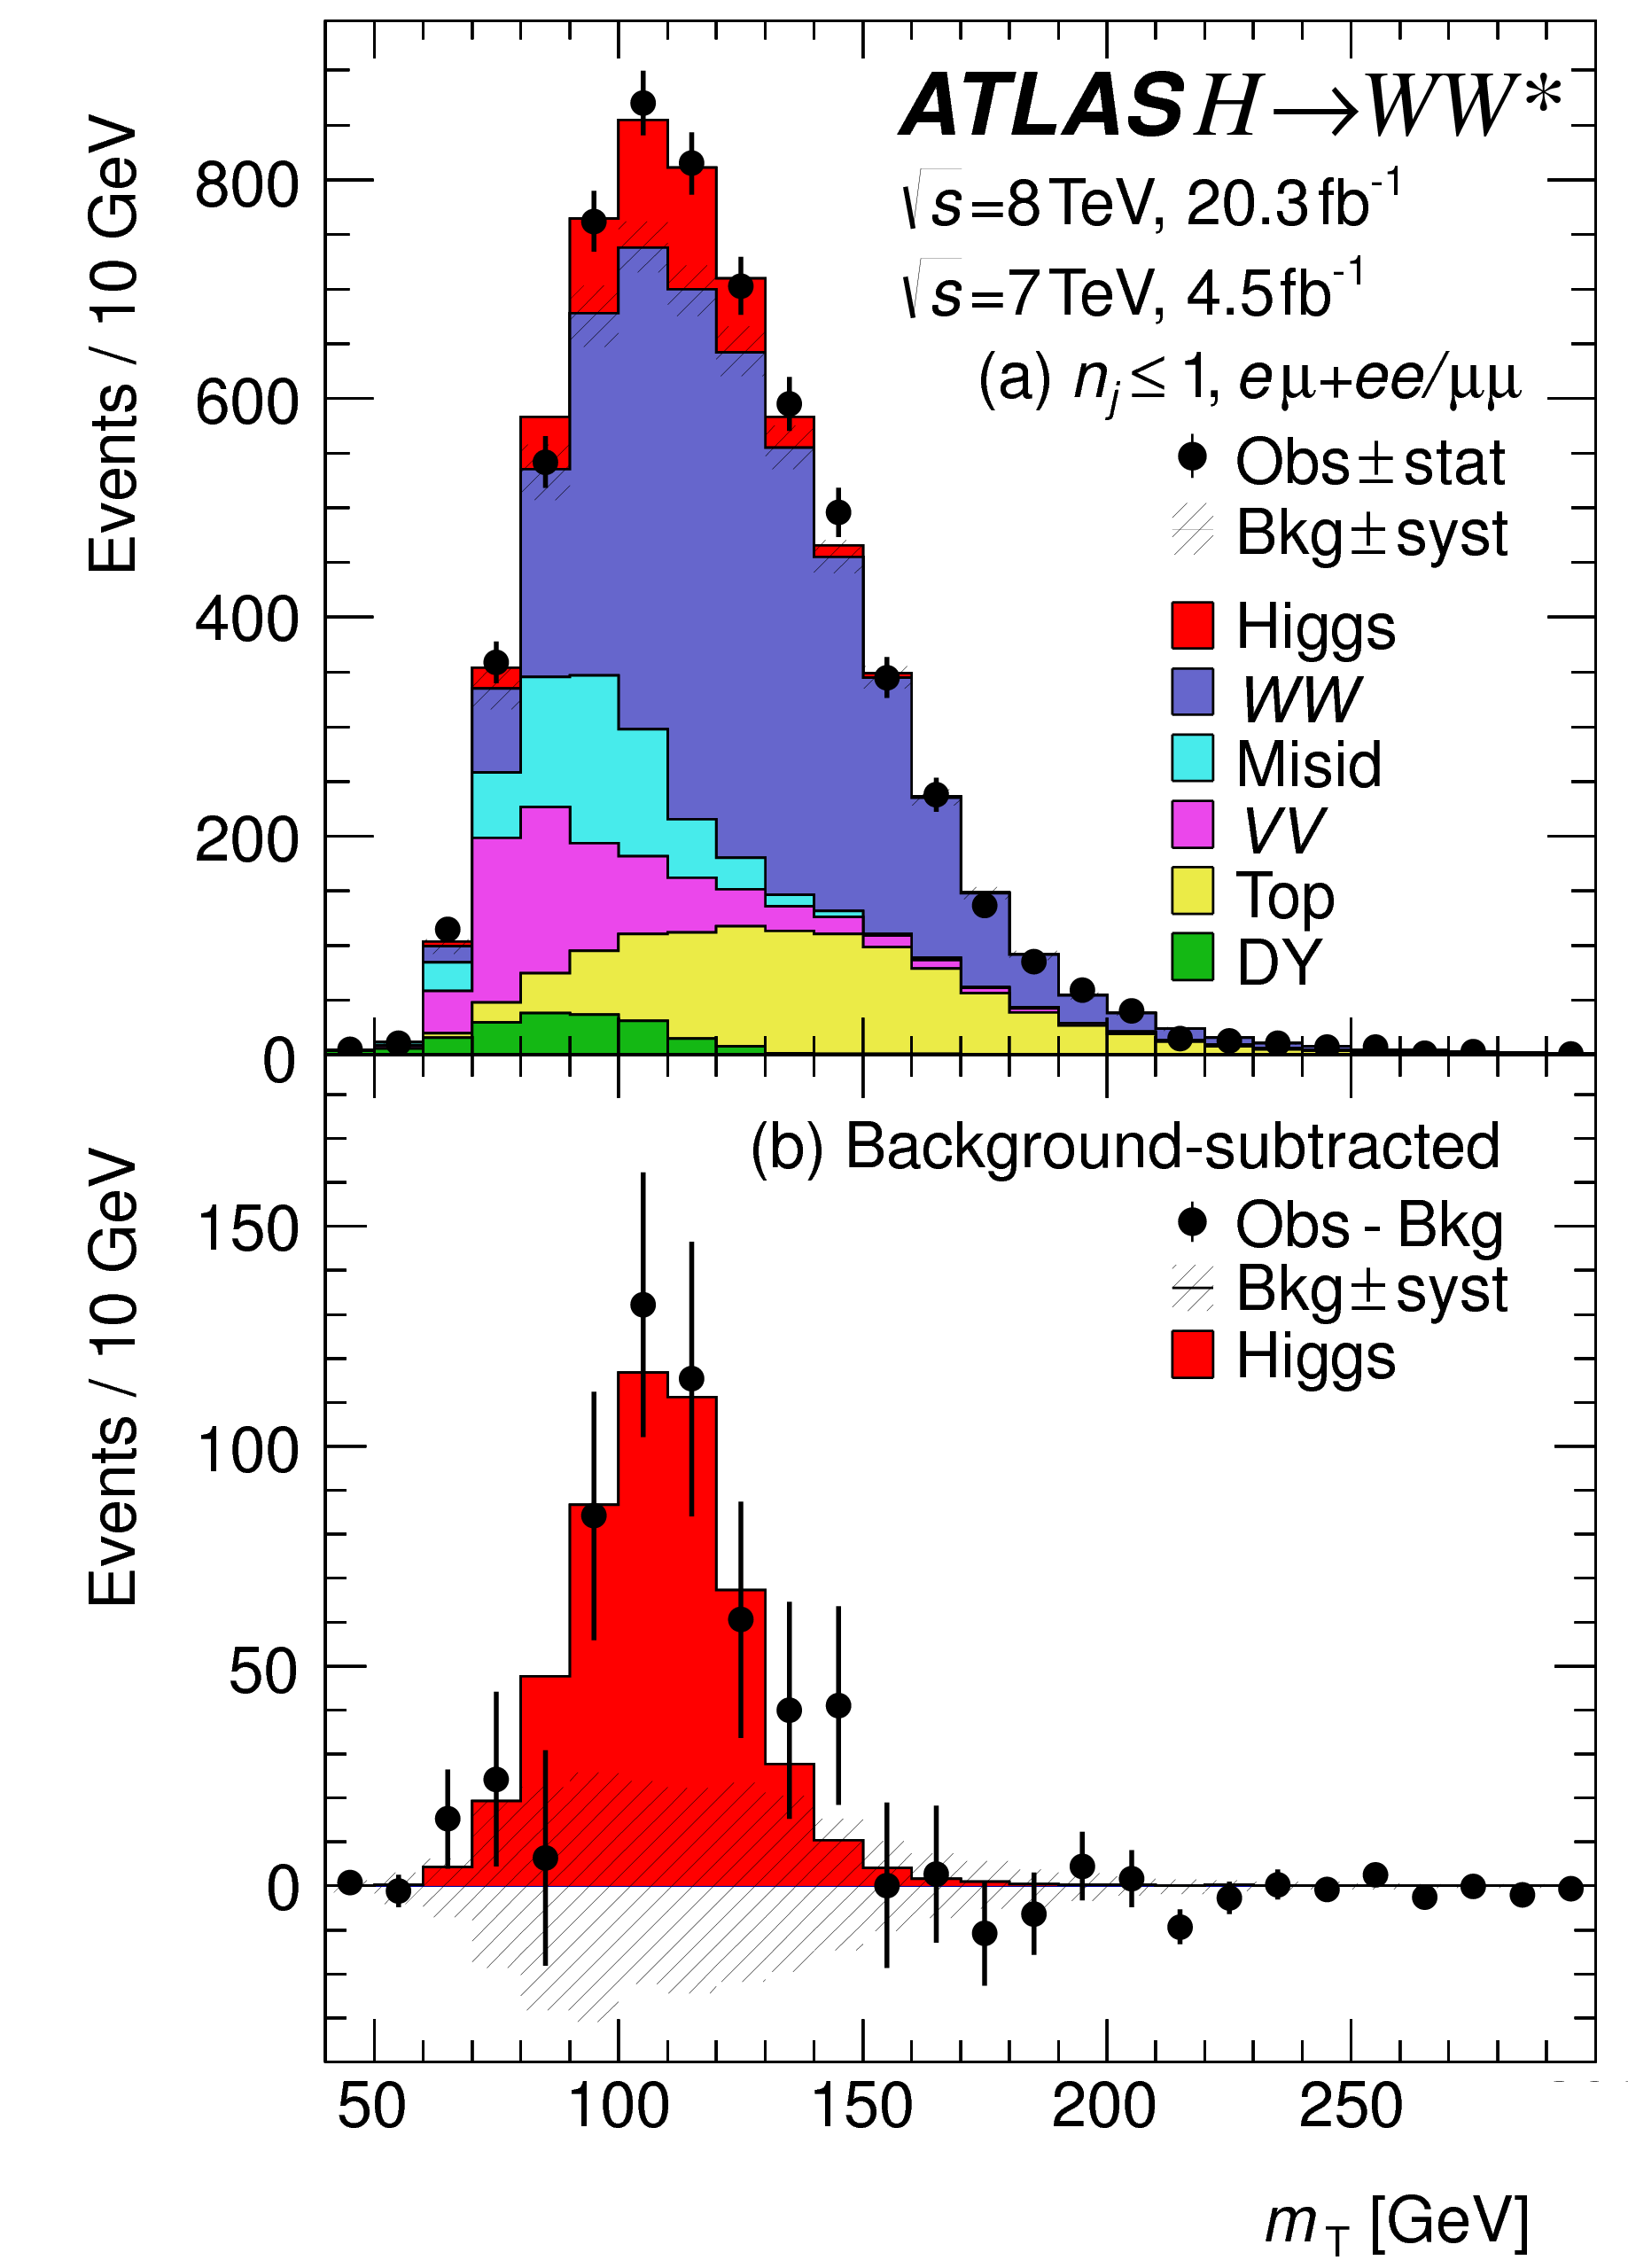
\includegraphics[width=0.6\textwidth]{figures/ggF_mT}
  \caption{Post-fit $\mTH$ distribution in the $\Njet \leq 1$ regions~\cite{WW2015}.}
  \label{fig:ggF-mT}
\end{figure}
%
These yields are used as input, along with the VBF results in chapter 5, for the physical interpretation of results presented in subsequent sections. 

\section{Signal strength measurements in ggF and VBF production}

A combined measurement of the signal strength, as well as the individual ggF and VBF signal strengths, is extracted when all of the signal regions are combined in the fit. A total cross section for the combined gluon fusion and vector boson fusion Higgs processes is measured, and this sum is normalized to theory prediction to obtain a value for the combined signal strength. The final measured combined signal strength $\mu$ is
%
\begin{equation}
\begin{array}{llllll}
 \mu
 &= 1.09%
 &^{+0.16}_{-0.15}\,(\textrm{stat.})%
 &^{+0.08}_{-0.07}\,\Big(\!\begin{tabular}{c}{\rm\footnotesize expt}\\ \noalign{\vskip -0.50truecm}{\rm\footnotesize syst}\end{tabular}\!\Big)%
 &^{+0.15}_{-0.12}\,\Big(\!\begin{tabular}{c}{\rm\footnotesize theo}\\ \noalign{\vskip -0.50truecm}{\rm\footnotesize syst}\end{tabular}\!\Big)%
 &{\PM}0.03\,\Big(\!\begin{tabular}{c}{\rm\footnotesize lumi}\\ \noalign{\vskip -0.50truecm}{\rm\footnotesize syst}\end{tabular}\!\Big)%
 \\
 \clineskip
 &= 1.09 &^{+0.16}_{-0.15}\,\textrm{(stat)} &^{+0.17}_{-0.14}\,\textrm{(syst)}
 \\
 \clineskip
 \clineskip
 &= 1.09 &^{+0.23}_{-0.21}.
\end{array}
\label{eqn:final-mu}
\end{equation}
%
Figure~\ref{fig:mu-val} gives the best fit signal strength $\hat{\mu}$ as a function of the hypothesized Higgs mass. The value at a mass of $125.36 \GeV$ corresponds to the $\mu$ quoted in equation~\ref{eqn:final-mu}. This value of the Higgs mass is used because it is the most precise mass measurement from ATLAS, a result of the combined $\gamma\gamma$ and $ZZ$ mass measurements~\cite{HiggsMass}. The figure also illustrates that the \HWWfull channel would have been sensitive to the Higgs boson at higher masses as well\footnote{A $\mu$ far below unity at higher masses indicates that there were many more expected events than were observed.}. 

\begin{figure}[h!]
  %\vspace{20pt}
  \centering
  \captionsetup{justification=centering}

  %\hspace*{-32pt}
  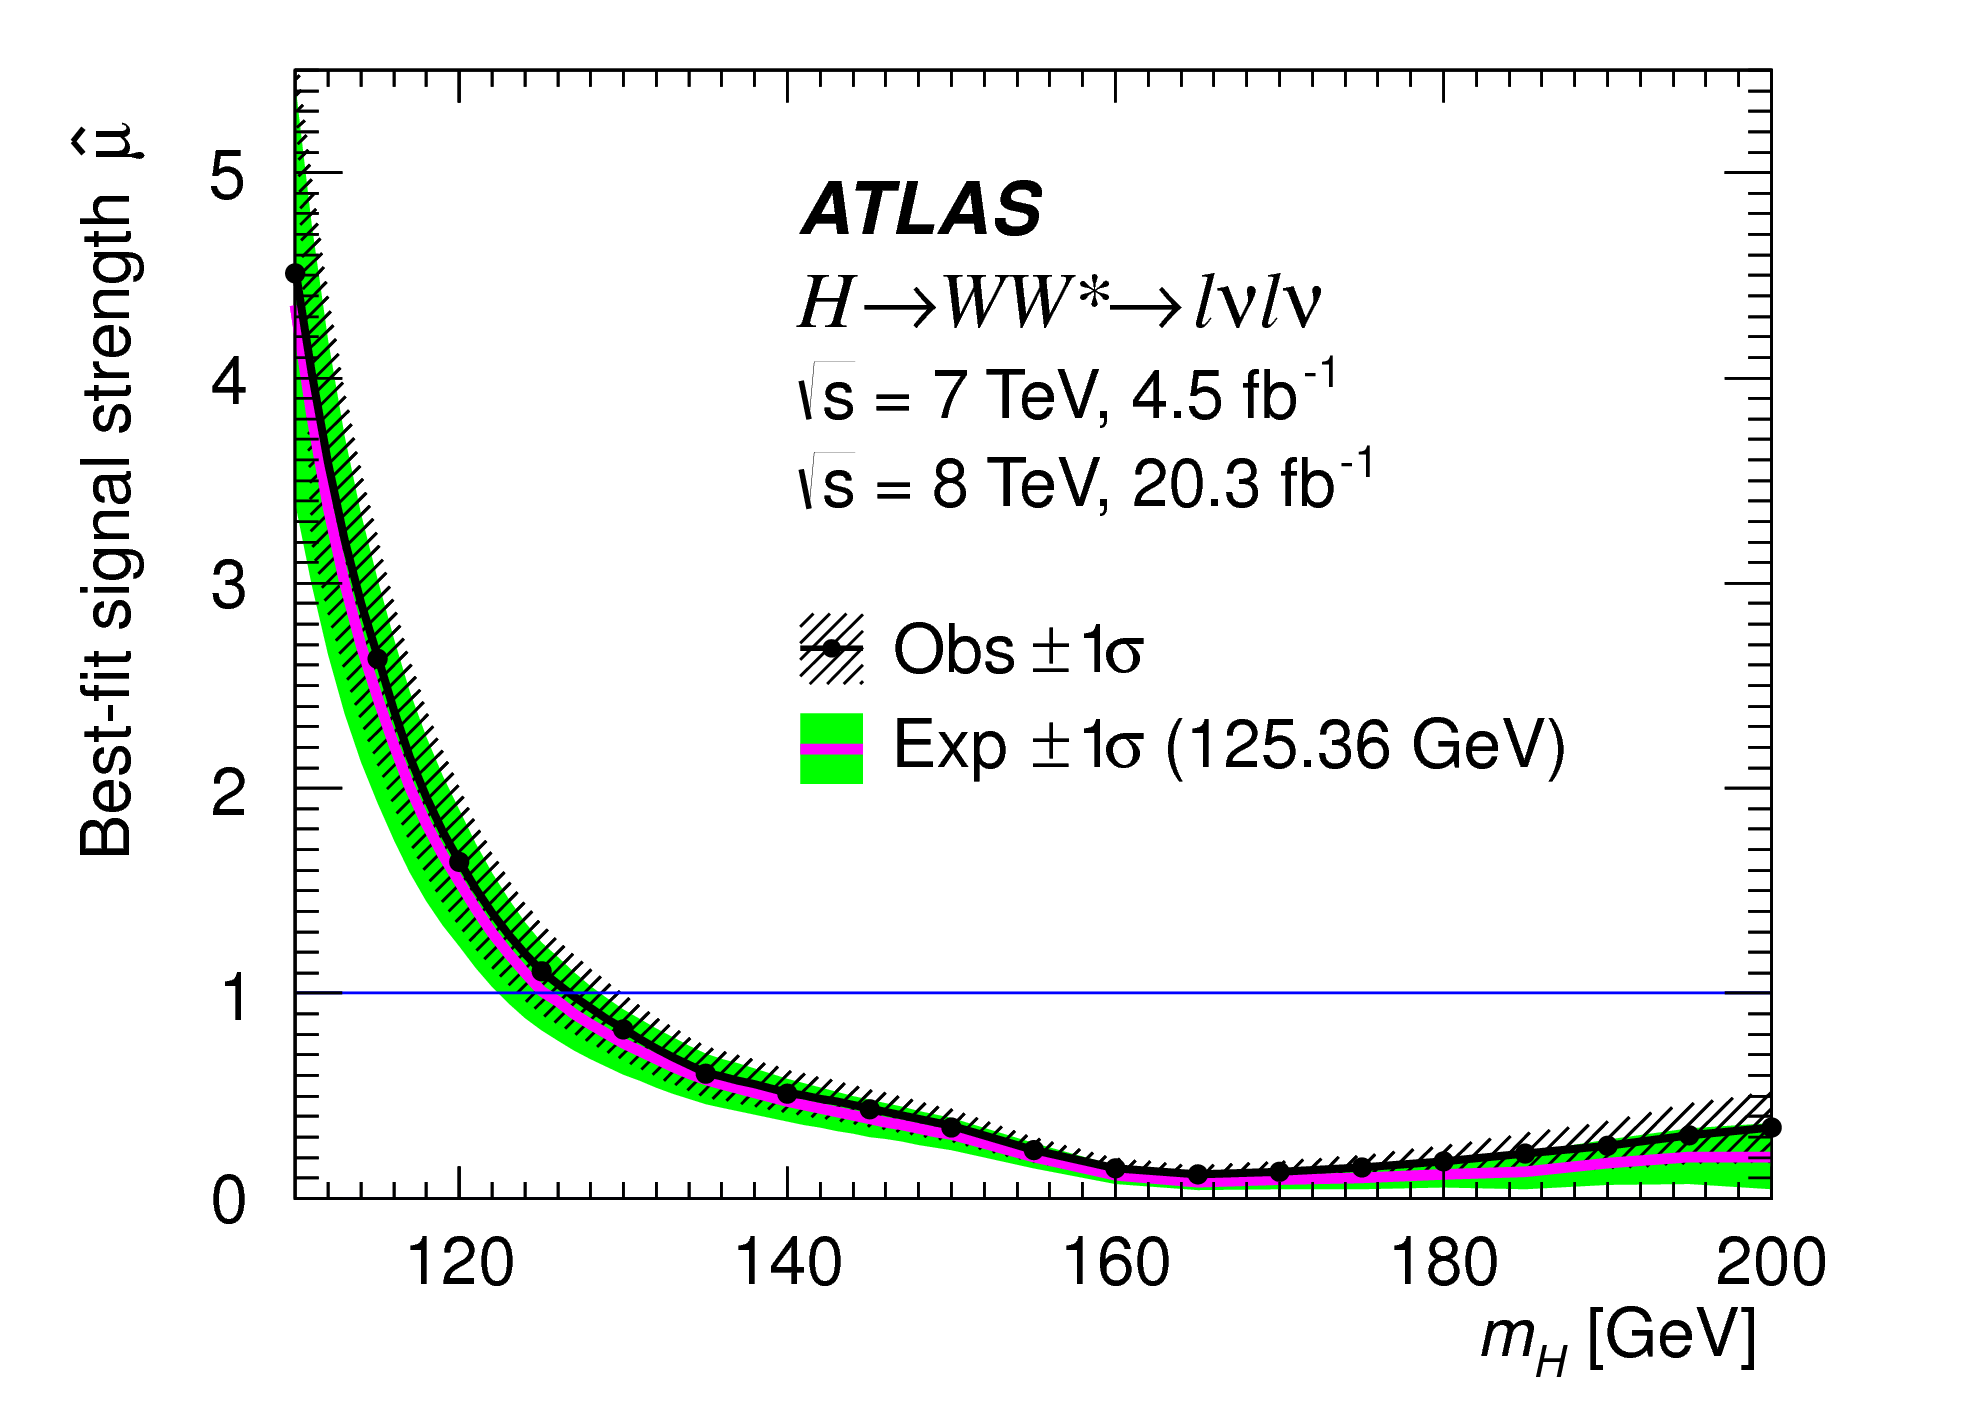
\includegraphics[width=0.7\textwidth]{figures/mu_mass}
  \caption{Best fit signal strength $\hat{\mu}$ as a function of hypothesized $m_{H}$~\cite{WW2015}.}
  \label{fig:mu-val}
\end{figure}

As explained in chapter 3, a probability $p_0$ can be computed using the test statistic $q_0$ to quantify the probability that the background could fluctuate to produce an excess at least as large as the one observed in the data. The local $p_0$ value is shown in figure~\ref{fig:p0} as a function of $m_H$. The minimum $p_0$ value is at $m_H = 130 \GeV$ and corresponds to a significance of $6.1\sigma$. The curve is relatively flat and the significance is the same at $125.36 \GeV$ within the quoted precision. The expected significance for a signal with strength $\mu = 1.0$ is $5.8\sigma$. This represents the first discovery level observation of Higgs production using only the \HWWfull analysis. 

\begin{figure}[h!]
  %\vspace{20pt}
  \centering
  \captionsetup{justification=centering}

  %\hspace*{-32pt}
  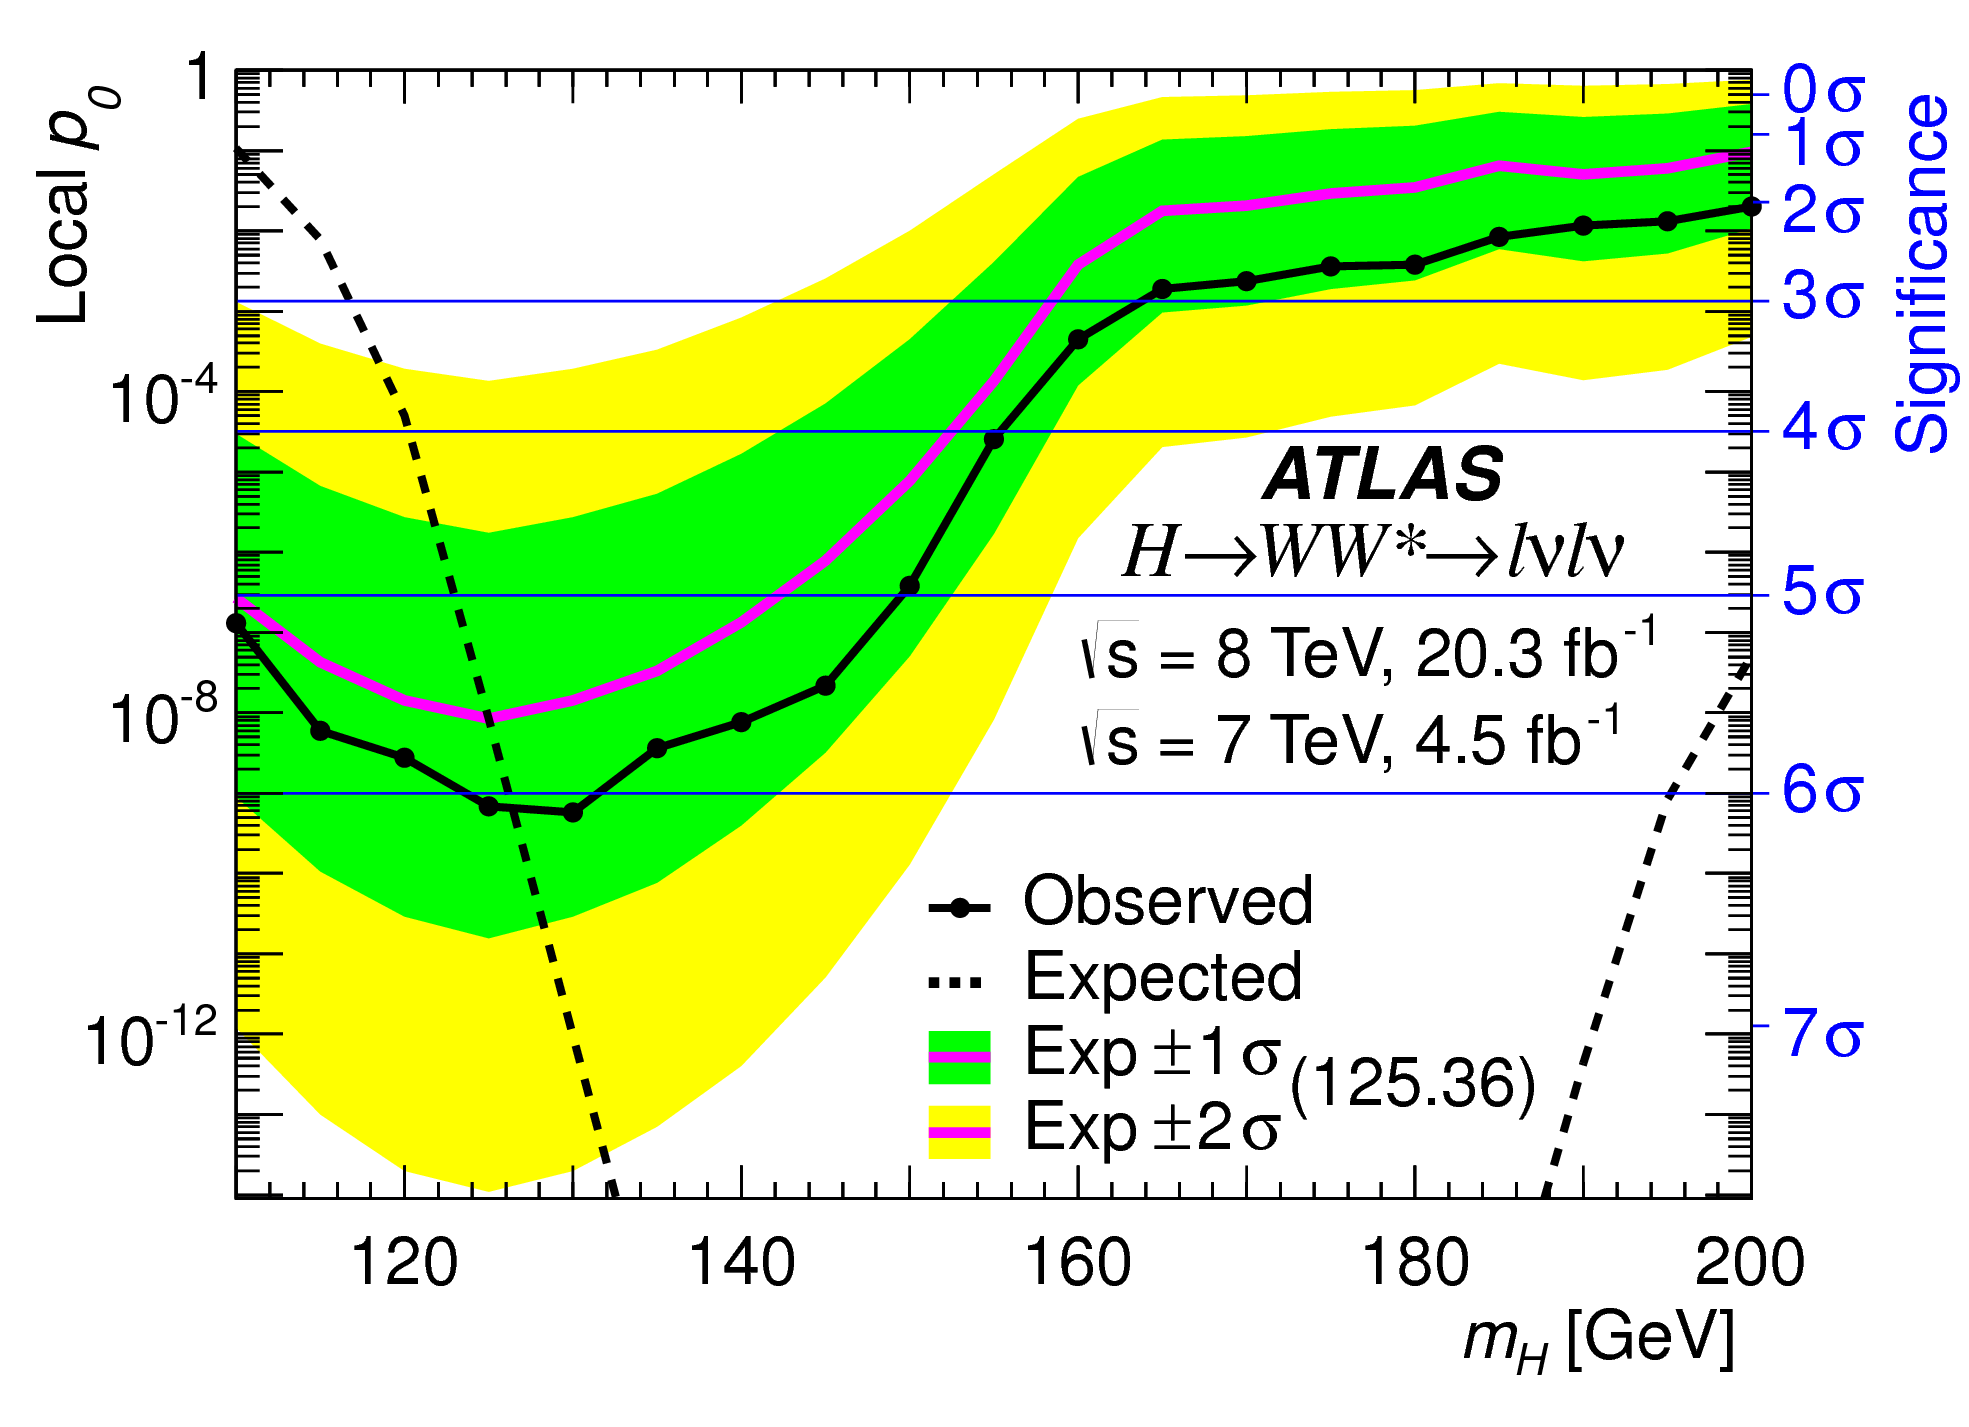
\includegraphics[width=0.7\textwidth]{figures/WW_p0}
  \caption{Local $p_0$ as a function of $m_H$~\cite{WW2015}.}
  \label{fig:p0}
\end{figure}

All the results presented so far in this section have been for the combined gluon fusion and VBF production modes. However, each signal strength can be calculated separately in the likelihood as well. There are two ways to do this. First, the likelihood can be parameterized in terms of a single parameter, the ratio of the VBF and gluon fusion signal strengths. With this method, the statistical significance of the VBF Higgs result can be evaluated. Figure~\ref{fig:mu_ratio} shows the likelihood as a function of the ratio $\mu_{\VBF}/\mu_{\ggF}$.
%
\begin{figure}[h!]
  %\vspace{20pt}
  \centering
  \captionsetup{justification=centering}

  %\hspace*{-32pt}
  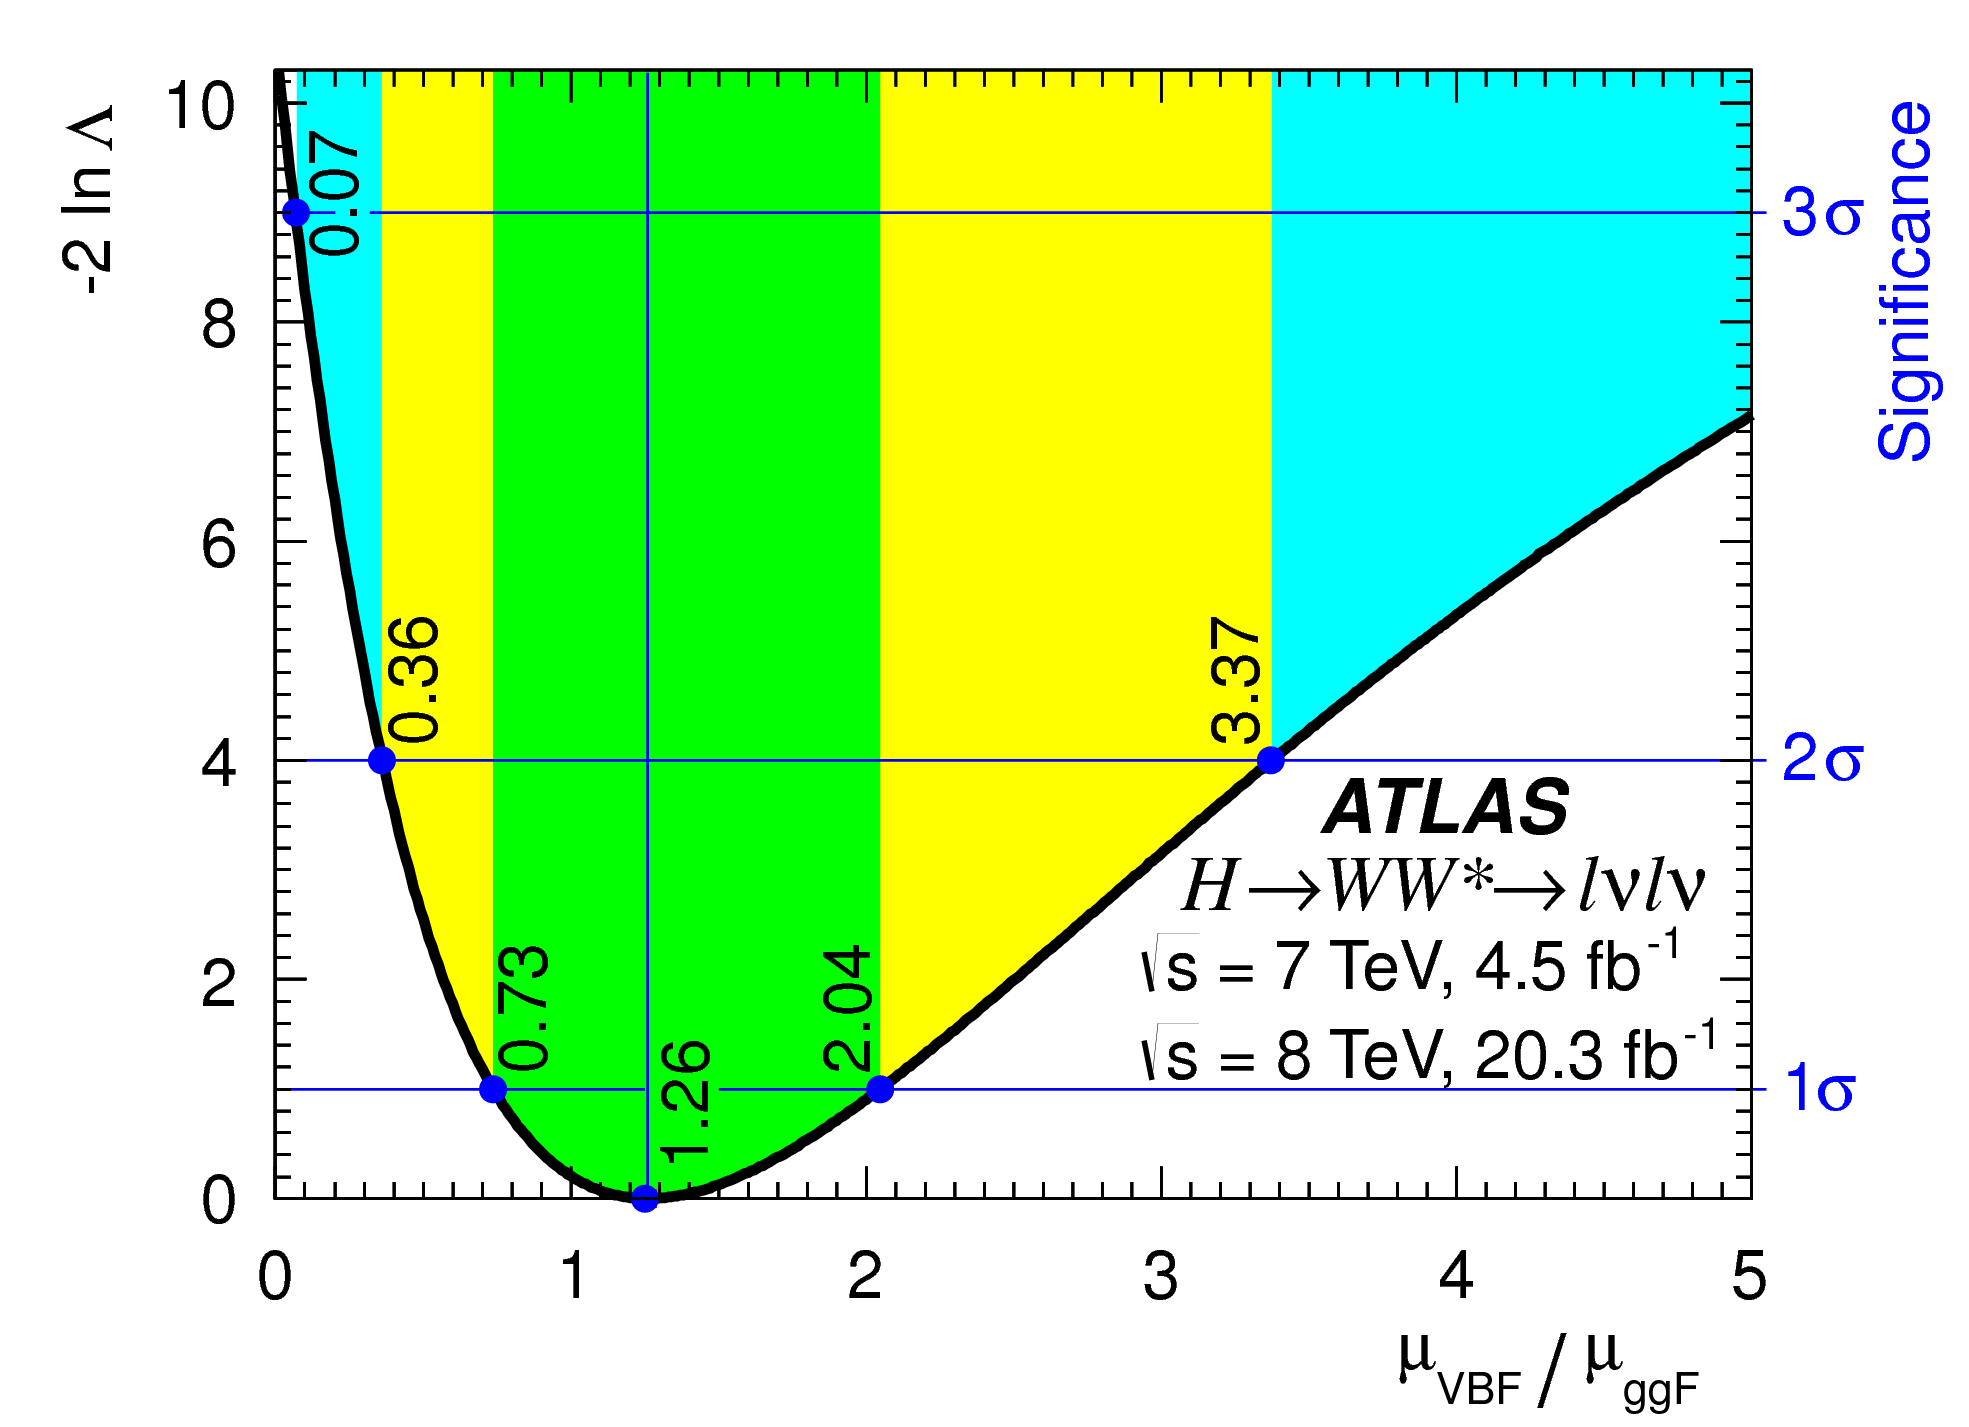
\includegraphics[width=0.7\textwidth]{figures/WW_muratio}
  \caption{Likelihood as a function of $\mu_{\VBF}/\mu_{\ggF}$~\cite{WW2015}.}
  \label{fig:mu_ratio}
\end{figure}
%
The best fit value of the ratio of signal strengths is shown in equation~\ref{eqn:mu_ratio}. Within the quoted uncertainties, it is consistent with a ratio of unity. 
%
\begin{equation}
  \frac{\mu_{\scVX}}{\mu_{\scggF}} 
  = 1.26\,^{+0.61}_{-0.45}\,(\rm{stat.})\,^{+0.50}_{-0.26}\,(\rm{syst.})
  = 1.26\,^{+0.79}_{-0.53} 
\label{eqn:mu_ratio}
\end{equation}
%
The null hypothesis for VBF production corresponds to a ratio of $\mu_{\VBF}/\mu_{\ggF} = 0$. The likelihood in figure~\ref{fig:mu_ratio} gives a significance of $3.2\sigma$ at $\mu_{\VBF}/\mu_{\ggF} = 0$, as quoted in chapter 5. 

In addition to the ratio of signal strengths, each signal strength can be varied independently in the likelihood as well. Figure~\ref{fig:mu_2d} shows the two dimensional likelihood scan in the $\mu_{\ggF}$-$\mu_{\VBF}$ plane. The best fit values of the two signal strengths are shown in equation~\ref{eqn:mu_ind}. Both are consistent with unity within their uncertainties.
%
\begin{equation}
\begin{array}{llllll}
\no\mu_{\scggF}\no&=1.02\no&{\PM}0.19           \np&^{+0.22}_{-0.18}\np&=1.02&^{+0.29}_{-0.26} \\ \clineskip
\no\mu_{\scVX} \no&=1.27\no&\,\,^{+0.44}_{-0.40}\np&^{+0.29}_{-0.21}\np&=1.27&^{+0.53}_{-0.45}.\\ \clineskip
                     &        & ~\textrm{(stat.)}     &\textrm{(syst.)}\np
\end{array}
\label{eqn:mu_ind}
\end{equation}

\begin{figure}[h!]
  %\vspace{20pt}
  \centering
  \captionsetup{justification=centering}

  %\hspace*{-32pt}
  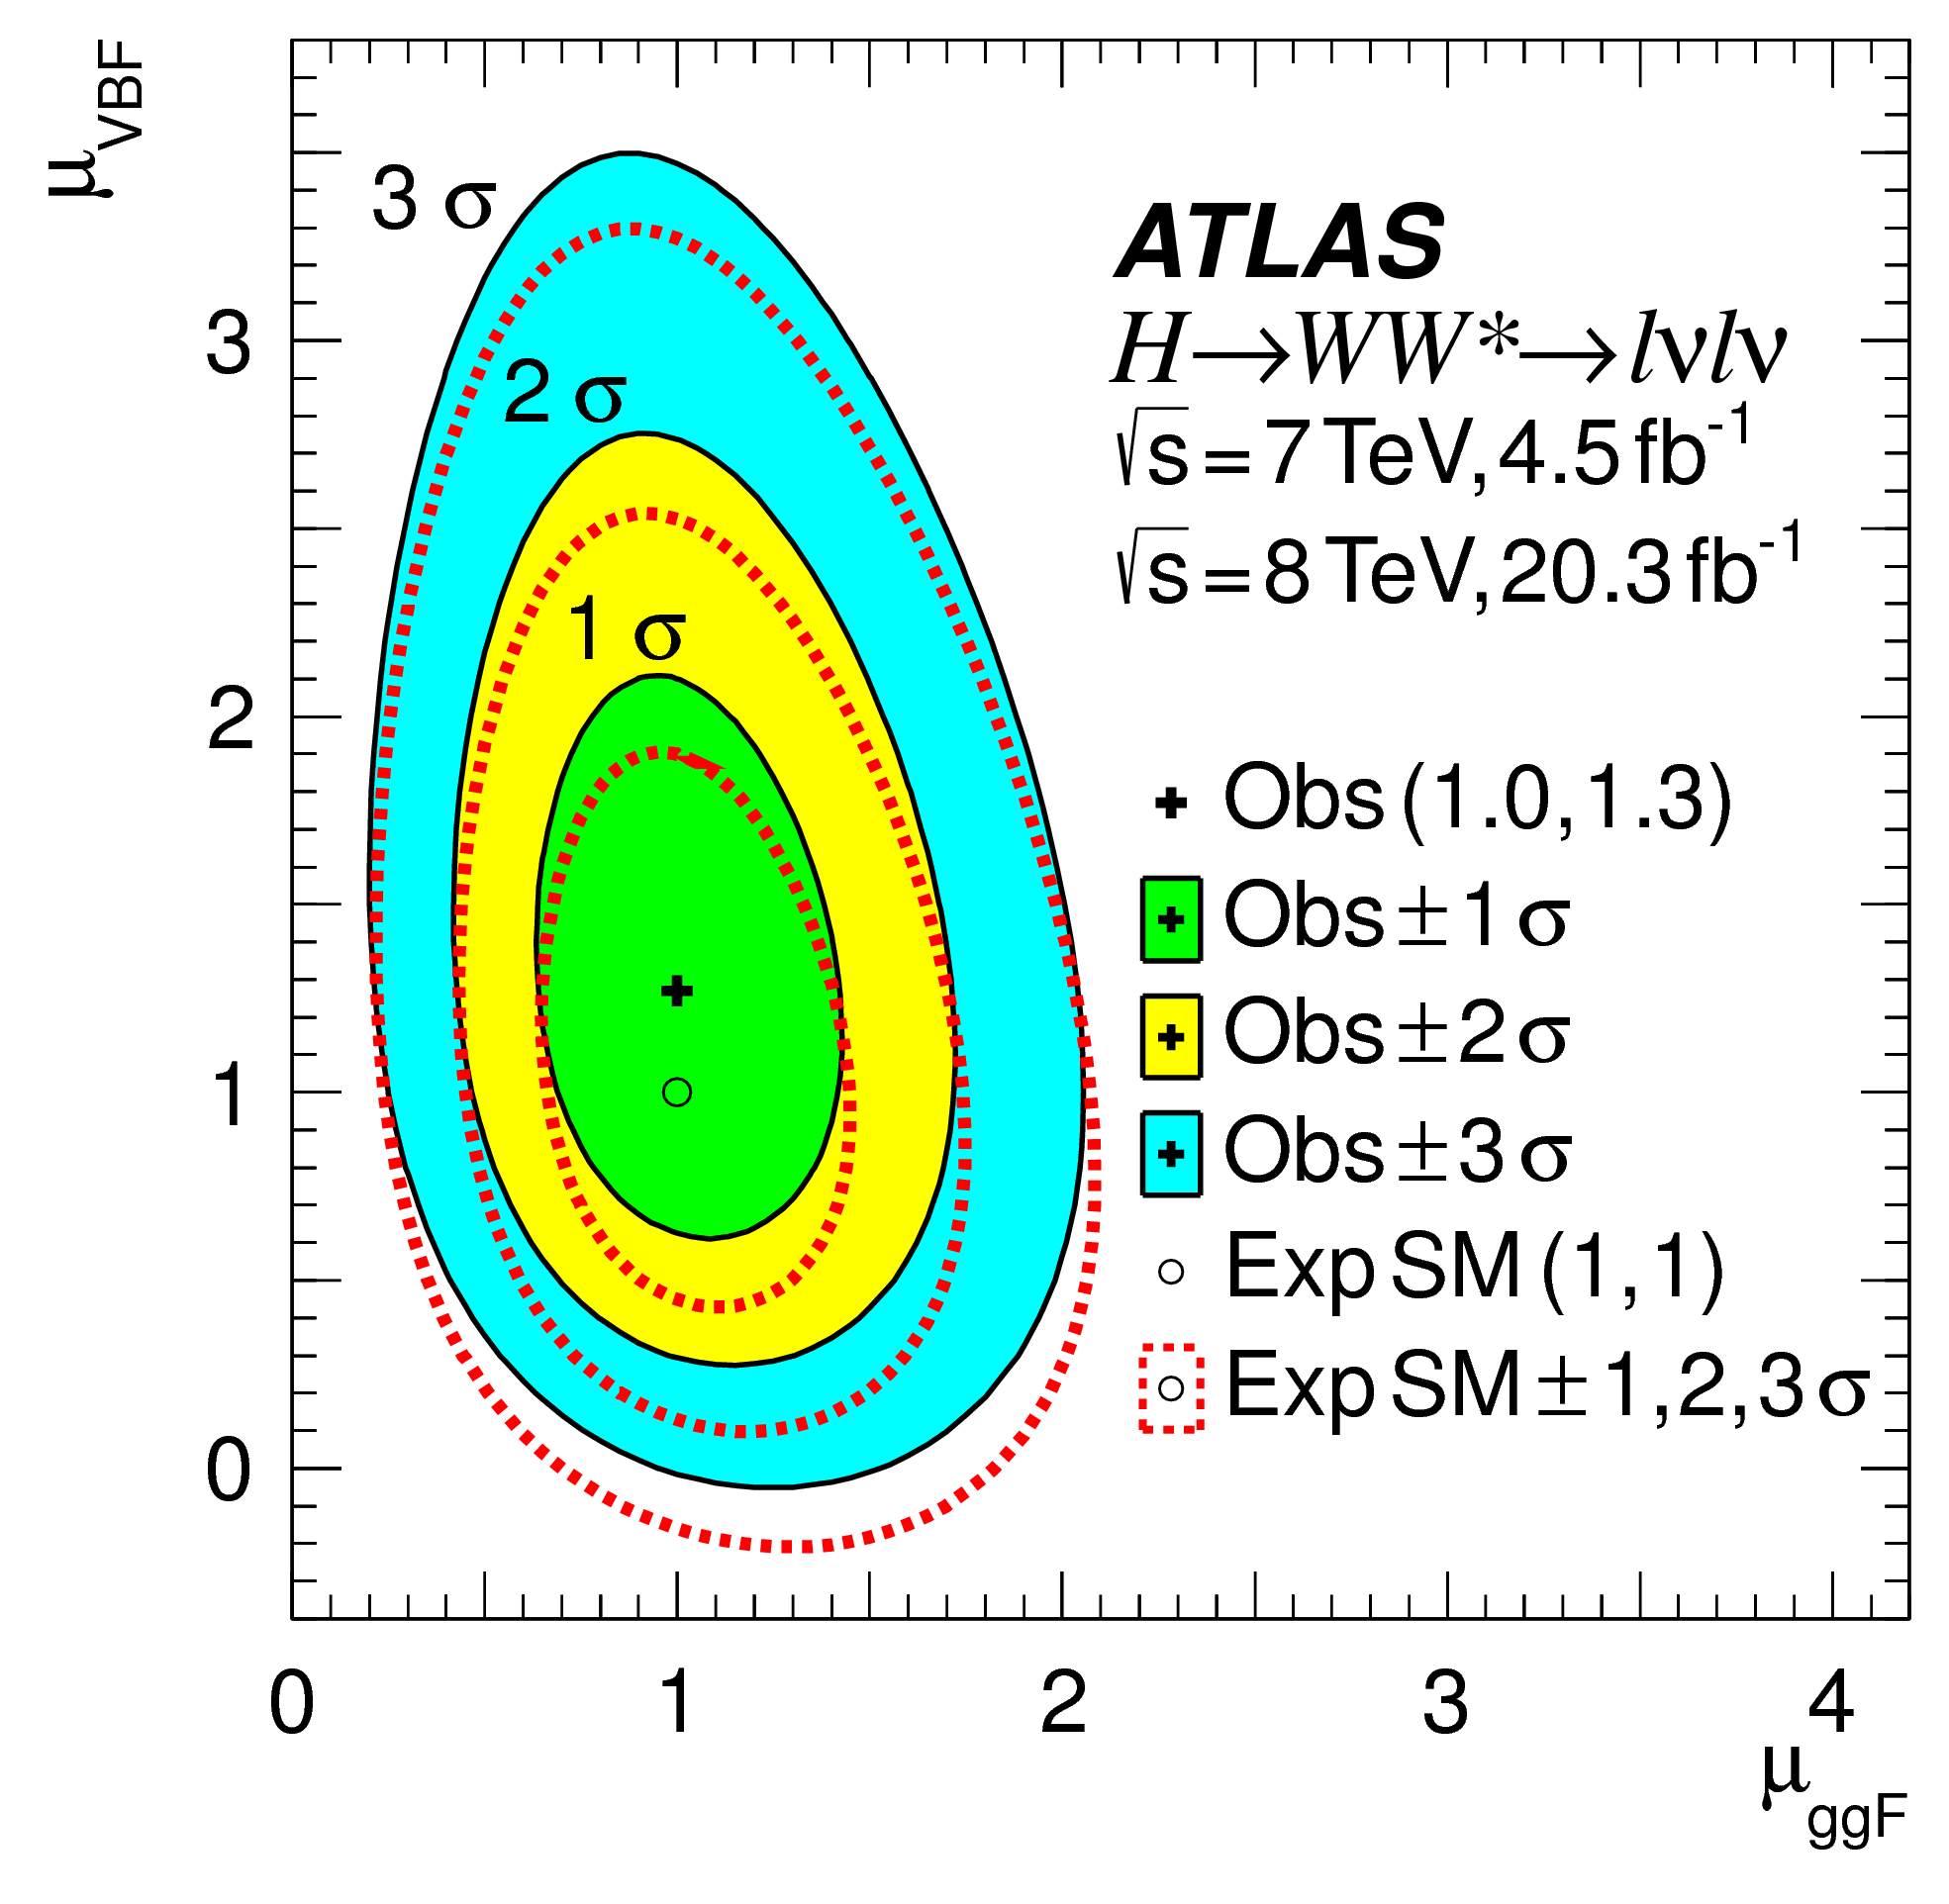
\includegraphics[width=0.7\textwidth]{figures/WW_muind}
  \caption{Two dimensional likelihood scan as a function of $\mu_{\VBF}$ and $\mu_{\ggF}$~\cite{WW2015}.}
  \label{fig:mu_2d}
\end{figure}

\section{Measurement of Higgs couplings to vector bosons and fermions}

The couplings of the Higgs to fermions and bosons are also measured relative to theoretical prediction. The parameter of interest in this case is referred to as $\kappa$, or the ratio of the measured coupling to the Standard Model expectation\footnote{$\kappa$ is to coupling measurements what $\mu$ is to cross section measurements.}. Both the fermion and boson couplings have these so-called scale factors, $\kF$ for fermions and $\kV$ for bosons. Gluon fusion production is sensitive to the fermion couplings through the top quark loops in its production, while VBF production is sensitive to the vector boson couplings in its production. Both modes are sensitive to the vector boson couplings in their decays. The signal strengths will have dependence on the coupling scale factors~\cite{LHCXSWG}. 
%
\begin{equation}
\np%
\begin{array}{lc l}
  \mu_{\scggF} &\propto &{\displaystyle\frac{\kF^2 \cdot \kV^2}{(\BF_{\Hff}+\BF_{\Hgg})\,\kF^2+(\BF_{\HVV})\,\kV^2}}\\ \clineskip\clineskip
  \mu_{\scVBF} &\propto &{\displaystyle\frac{\kV^4            }{(\BF_{\Hff}+\BF_{\Hgg})\,\kF^2+(\BF_{\HVV})\,\kV^2}} . 
\end{array}
\label{eqn:kappas}
\end{equation}
%
Figure~\ref{fig:kappas} shows the two-dimensional likelihood scan of $\kF$ and $\kV$. The best-fit values are given in equation~\ref{eqn:kappa_vals}. The best-fit values are consistent with unity within their uncertainties. 
%
\begin{equation}
\begin{array}{llllll}
\no\kF\no&=0.93\no&\,\,^{+0.24}_{-0.18}\np&^{+0.21}_{-0.14}\np&=0.93&^{+0.32}_{-0.23} \\ \clineskip
\no\kV\no&=1.04\no&\,\,^{+0.07}_{-0.08}\np&^{+0.07}_{-0.08}\np&=1.04&{\PM}0.11.\\ \clineskip
                     &        & ~\textrm{(stat.)}     &\textrm{(syst.)}\np
\end{array}
\label{eqn:kappa_vals}
\end{equation}
%
\begin{figure}[h!]
  %\vspace{20pt}
  \centering
  \captionsetup{justification=centering}

  %\hspace*{-32pt}
  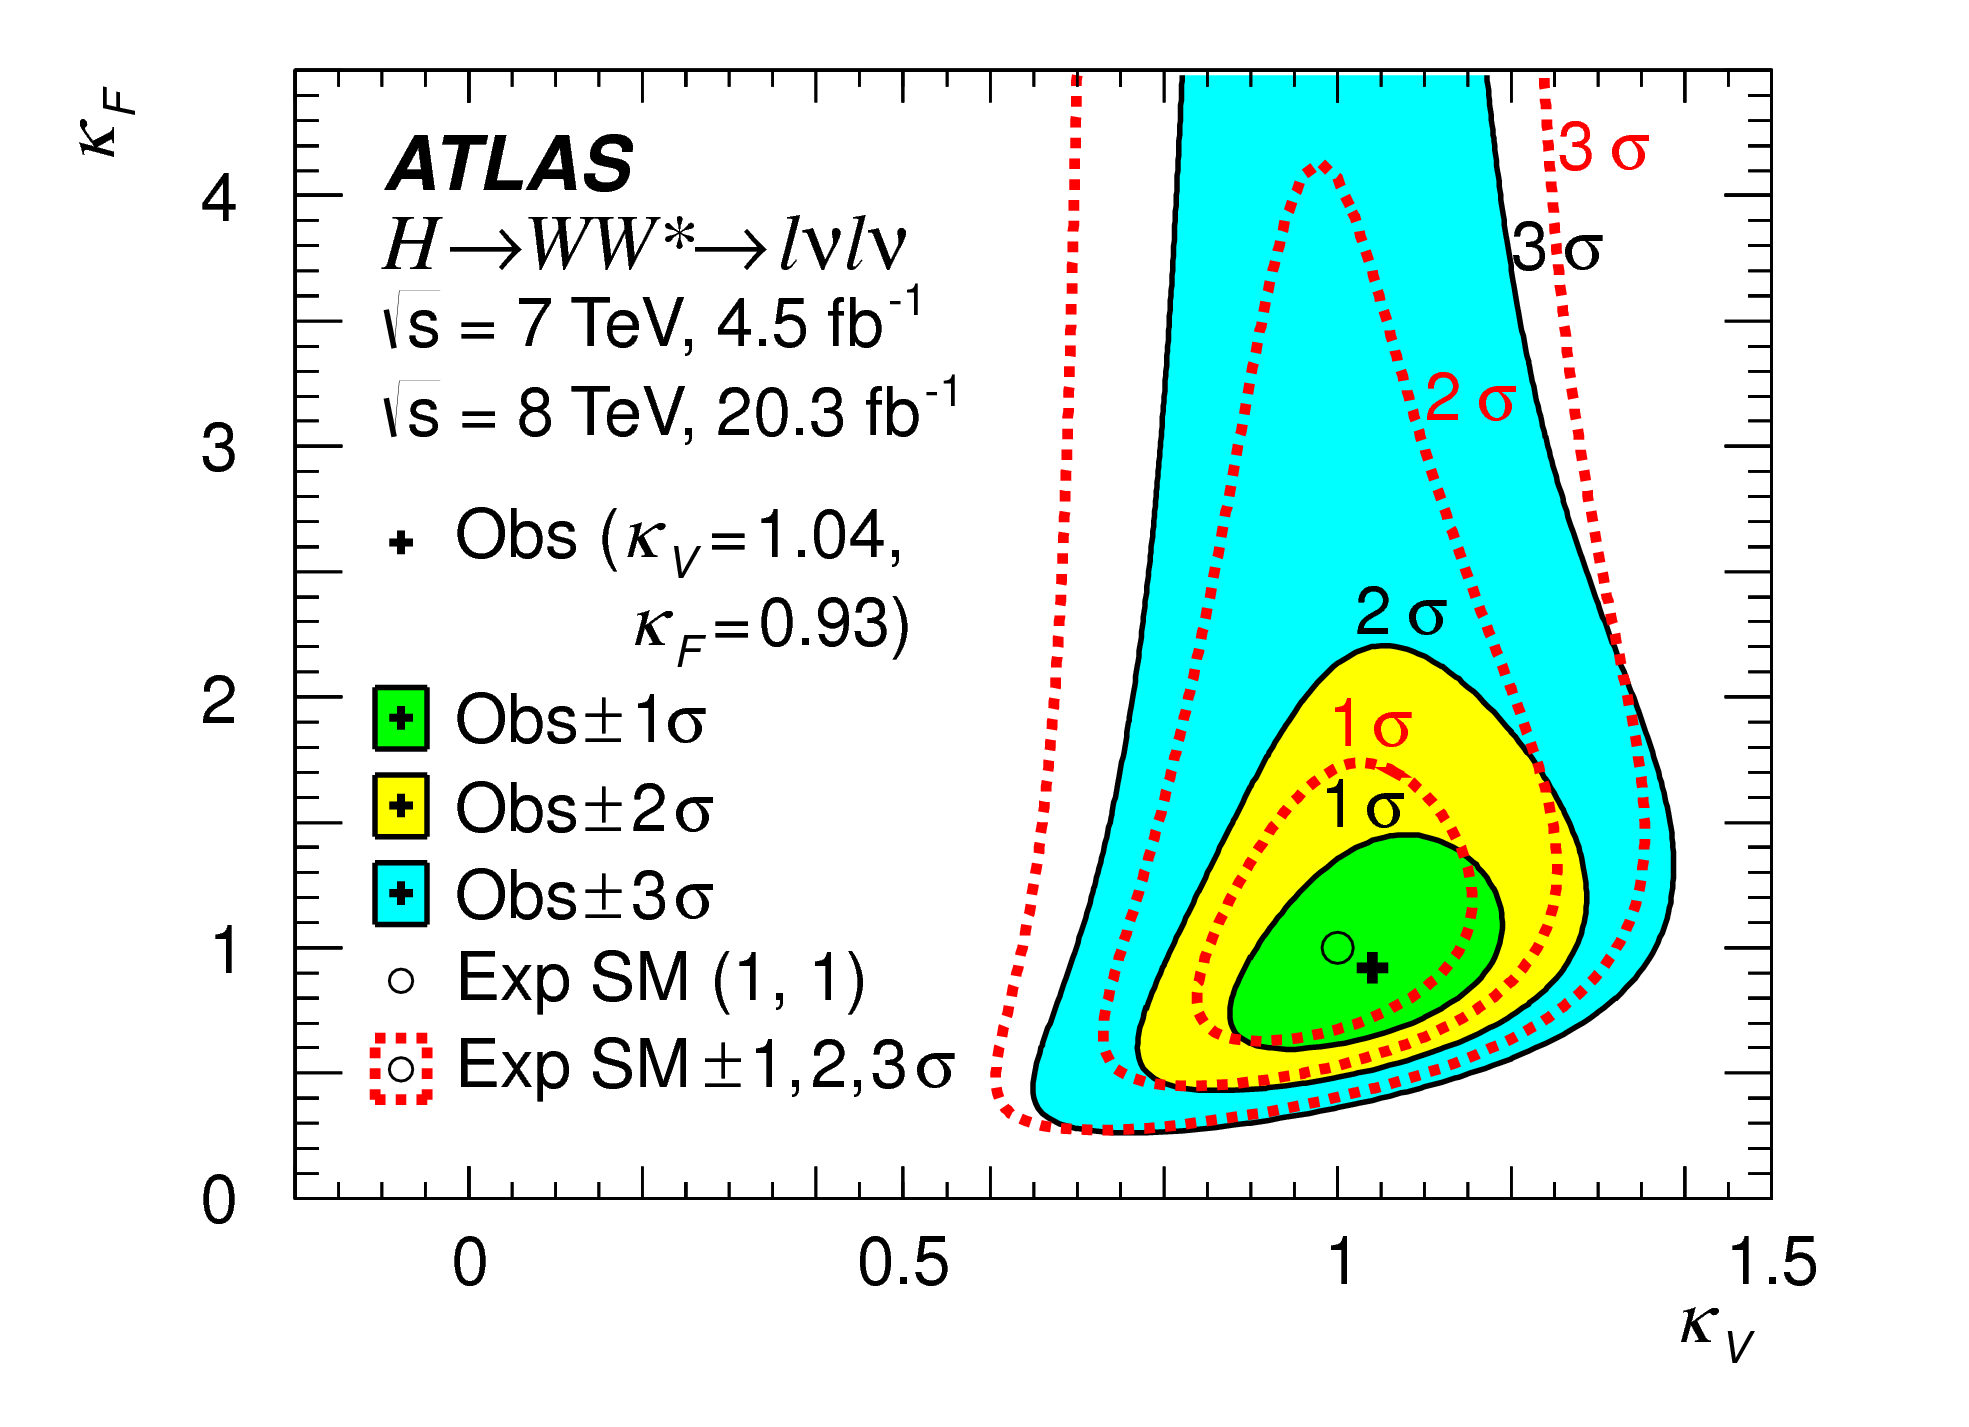
\includegraphics[width=0.7\textwidth]{figures/kappas}
  \caption{Likelihood scan as a function of $\kF$ and $\kV$, the Higgs coupling scale factors~\cite{WW2015}.}
  \label{fig:kappas}
\end{figure}

\section{Higgs production cross section measurement}

Another measurement that comes naturally from the signal strength measurements quoted earlier is the production cross section at $7$ and $8 \TeV$ for both gluon fusion and VBF production. The general equation for calculating the cross section is
%
\begin{equation}
\begin{array}{ll}
\nq\big(\sigma \cdot\mathcal{B}_{\HWW}\big)_\obs
&=
\frac{\displaystyle (\Nsig)_\obs}
     {\displaystyle \Acc\cdot\Cor\cdot\mathcal{B}_{WW\rightarrow \ell\nu\ell\nu}^{\phantom{X}}}
\cdot
\frac{\displaystyle 1}{\displaystyle\Lint} \\
\clineskip
\clineskip
&= 
{\displaystyle \hat{\mu} \cdot (\sigma\cdot\mathcal{B}_{\HWW})_\exp}.
\end{array}
\label{eqn:xsec}
\end{equation}
%
Here, $(\Nsig)_\obs$ is the number of events observed in data. $\Acc$ is the geometric and kinematic acceptance of the detector, while $\Cor$ is the efficiency of the signal region selection for events that are reconstructed in the detector. The branching ratio of a $WW$ system to leptons must also be divided out. The production cross section depends on the center of mass energy and the production mode desired (gluon fusion or VBF), and so three separate cross section measurements are obtained:
%
\begin{equation}
\begin{array}{lllllll}
\np\sigma_{\scggF}^{7\!\TeV}{\!\CDOT}\mathcal{B}_{\HWW}\np&= 2.0 \np\no&{\PM}1.7            \no\!&^{+1.2}_{-1.1}  \np\no&=2.0 \np\no&\,\,^{+2.1}_{-2.0}   \np&\pb \nq\\ \clineskip
\np\sigma_{\scggF}^{8\!\TeV}{\!\CDOT}\mathcal{B}_{\HWW}\np&= 4.6 \np\no&{\PM}0.9            \no\!&^{+0.8}_{-0.7}  \np\no&=4.6 \np\no&\,\,^{+1.2}_{-1.1}    \np&\pb \nq\\ \clineskip
\np\sigma_{\scVX }^{8\!\TeV}{\!\CDOT}\mathcal{B}_{\HWW}\np&= 0.51\np\no&\,\,^{+0.17}_{-0.15}\no\!&^{+0.13}_{-0.08}\np\no&=0.51\np\no&\,\,^{+0.22}_{-0.17} \np&\pb.\nq\\ \clineskip
\np                                                       &      \np\no&\textrm{(stat.)}    \no\!&\textrm{(syst.)}\np\no
\end{array}
\label{eqn:xsec_vals}
\end{equation}
%
These are the most precise measurements for the Higgs production cross sections from a single channel. The predicted cross section values (including the branching ratio of $\HWW$) for gluon fusion are $3.3 \pm 0.4 \pb$ at $7 \TeV$ and $4.2 \pm 0.5 \pb$ at $8 \TeV$, consistent with the measured values within their uncertainties. For vector boson fusion, the predicted cross section at $8 \TeV$ is $0.35 \pm 0.02 \pb$, again consistent with the measured value. 

\section{Conclusion}

The combined analysis of the gluon fusion and vector boson fusion processes in \HWWfull in the $7$ and $8 \TeV$ datasets has yielded the first discovery level significance for Higgs production in this decay channel. Additionally, precise measurements of the couplings to vector bosons and fermions were obtained. Finally, signal strengths and cross sections for each production mode were measured. Figure~\ref{fig:mu_summary} shows the \HWWfull measurements in comparison with other Higgs decay channels in ATLAS. The measurement of signal strength from this channel remains the most sensitive in both the gluon fusion and VBF production modes for the Run 1 dataset. 

\begin{figure}[h!]
  %\vspace{20pt}
  \centering
  \captionsetup{justification=centering}

  %\hspace*{-32pt}
  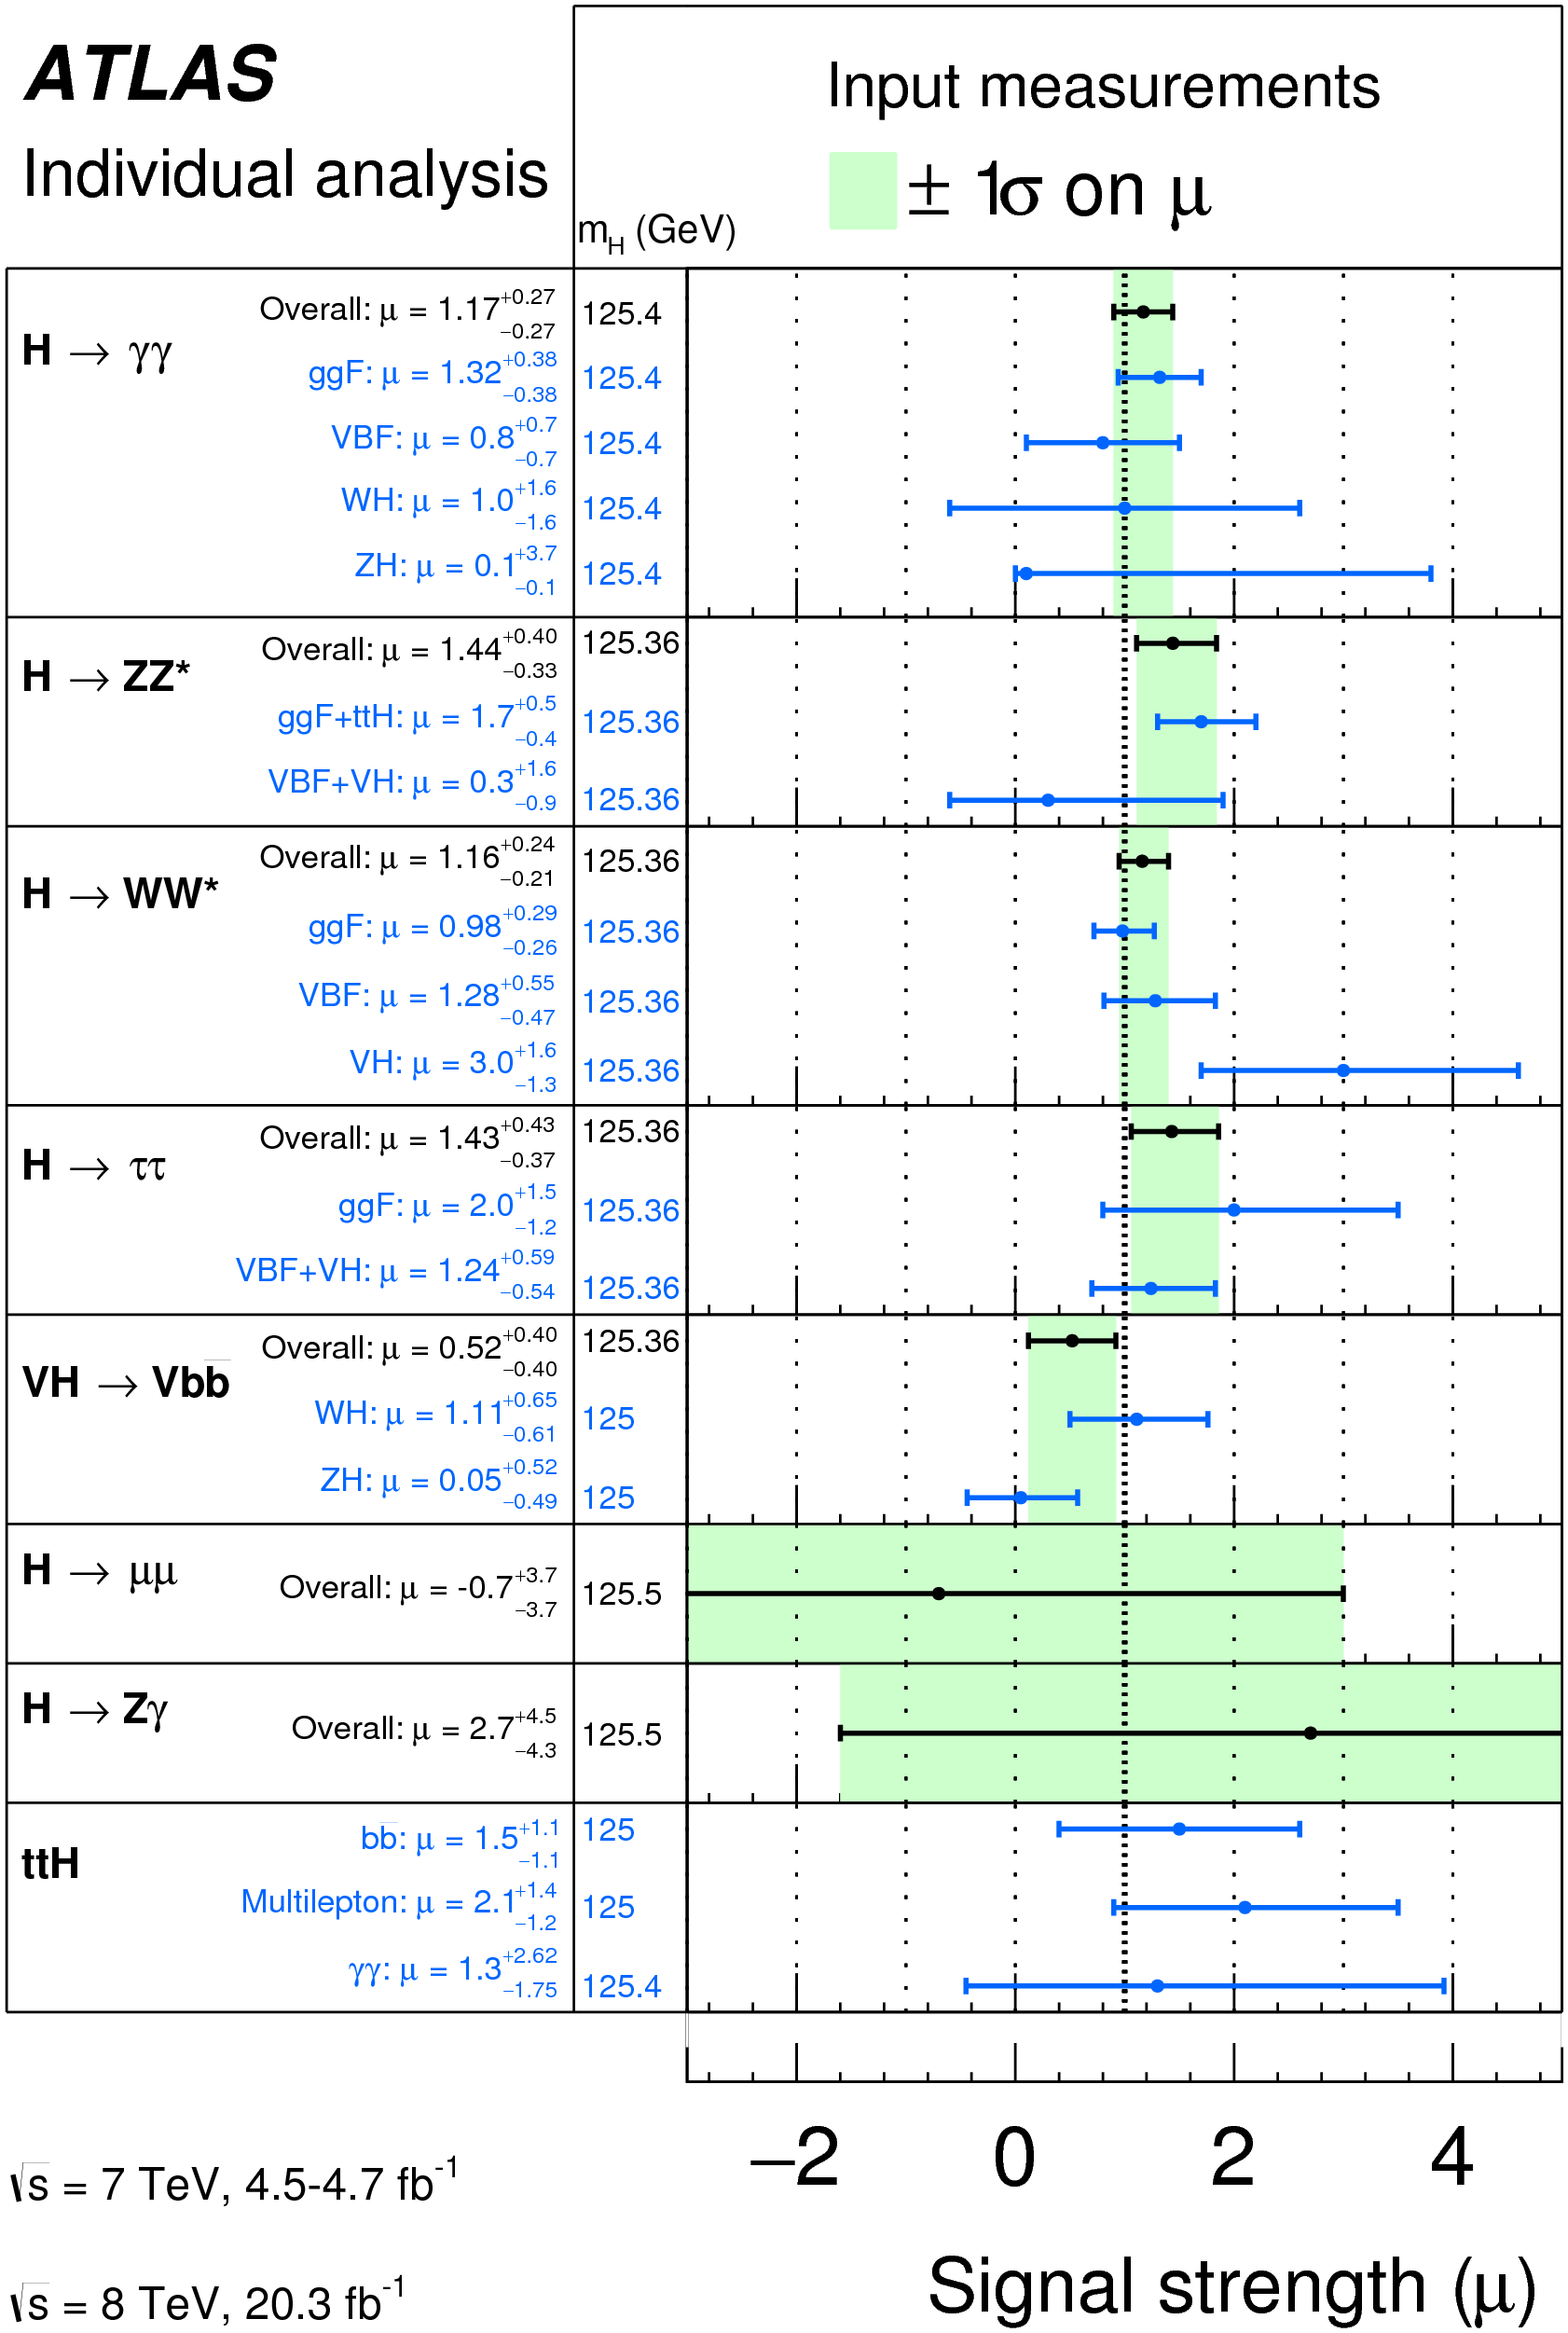
\includegraphics[width=0.7\textwidth]{figures/mu_summary}
  \caption{Comparison of signal strength measurements in different Higgs decay channels on ATLAS~\cite{HiggsSummaryRun1}.}
  \label{fig:mu_summary}
\end{figure}

